\documentclass[11pt]{article}

\usepackage[review]{acl}

\usepackage{times}
\usepackage{latexsym}
\usepackage[T1]{fontenc}
\usepackage[utf8]{inputenc}
\usepackage{microtype}
\usepackage{inconsolata}
\usepackage{graphicx}
\usepackage{booktabs}
\usepackage{amsmath}
\usepackage{amssymb}
\usepackage{url}

\title{QAPE: Quantization-Aware Prompt Evolution \\ for Quantized Small Language Models}

\author{Anonymous Authors \\
  Affiliation / Address line 1 \\
  \texttt{email@domain} \\}

\begin{document}
\maketitle

\begin{abstract}
Quantization is essential for deploying Small Language Models (SLMs) on resource-constrained edge devices. However, low-precision quantization (e.g., 4-bit) introduces behavioral and precision-induced drift, degrading model performance on complex reasoning and structured extraction tasks. We present \textbf{QAPE} (Quantization-Aware Prompt Evolution), a genetic algorithm-based prompt optimization framework that automatically recovers performance loss in quantized SLMs. Evaluating across four benchmarks (GSM8K, SVAMP, PII Anonymization, and Financial NER) on \texttt{Llama-3.2-3B} and \texttt{Qwen-2.5-0.5B}, we show that QAPE achieves significant performance gains (up to +25.0\% F1 recovery on Financial NER and +10.0\% accuracy on SVAMP). Furthermore, we analyze the \textit{cross-precision transferability} of evolved prompts, revealing that optimized prompts specialize to their target quantization level. Transferring prompts across precision boundaries (e.g., 4-bit to FP16) results in a minor performance penalty (6.67\% to 13.33\%) compared to direct optimization, though structured extraction tasks show high resilience to precision transfer.
\end{abstract}

\section{Introduction}
Small Language Models (SLMs) with sub-3B parameters enable local, privacy-preserving inference on consumer devices. To fit within unified memory limits, post-training quantization (PTQ) to 4-bit (Q4) is standard practice. While quantization reduces memory footprints, it introduces numerical drift that manifests as formatting failures, repetitive token loops, and degraded reasoning capability. 

Prior work has addressed this via quantization-aware training (QAT) or calibration. However, these methods are computationally expensive. We propose \textbf{QAPE} (Quantization-Aware Prompt Evolution), which uses a black-box genetic prompt optimization loop to mitigate precision degradation. QAPE uses a larger meta-model to iteratively mutate prompt candidates, selecting for high accuracy on the target quantized model.

We address two main research questions:
\begin{enumerate}
    \item \textbf{Degradation Recovery:} Can prompt evolution recover accuracy losses induced by quantization in sub-3B models?
    \item \textbf{Cross-Precision Transferability:} Do prompts evolved on a quantized target model (e.g., Q4) transfer to the full-precision version (e.g., FP16) and vice-versa, or do they specialize to the numerical characteristics of the specific precision?
\end{enumerate}

Our key contributions are three-fold:
\begin{itemize}
    \item We introduce \textbf{QAPE}, an automated black-box genetic prompt optimization framework specifically designed to address precision-induced drift in quantized SLMs.
    \item We demonstrate significant accuracy and F1 score recoveries (up to +25.02\% F1 recovery) across reasoning and structured extraction tasks for sub-3B and sub-1B models without parameter modification.
    \item We present a systematic study on the cross-precision transferability of evolved prompts, establishing that optimized templates specialize to their target numerical precision on math reasoning, while retaining robust formatting resilience on structured extraction.
\end{itemize}

\section{Related Work}
\paragraph{Post-Training Quantization (PTQ)}
Quantization techniques are critical for reducing the memory footprint of LLMs during deployment. Standard PTQ methods, such as GPTQ \cite{frantar2022gptq} and AWQ \cite{lin2023awq}, quantize weights to 4-bit or 3-bit precisions by optimizing for reconstruction loss on calibration data. For local deployments on CPU and unified memory architectures, GGUF formats under the \texttt{llama.cpp} framework are widely used. While PTQ successfully compresses models, it introduces numerical drift that degrades reasoning and structural compliance.

\paragraph{Precision-Induced Behavioral Drift}
Recent research has shown that low-precision models suffer from precision-induced behavioral drift, where the quantized model fails on tasks requiring strict formatting or multi-step logic. Google's Gemma 2 technical report \cite{gemma2} documents numerical instabilities in low-precision (FP16/Q4) regimes on specific hardware, driven by attention logit soft-capping mechanisms. Reconciling baseline scores reveals that these instabilities, combined with local hardware limitations (e.g., swapping latency and timeouts), can lead to anomalous performance drops that do not reflect the model's actual capability.

\paragraph{Black-Box Prompt Optimization}
Automated prompt engineering (APE) frameworks, such as DSPy \cite{khattab2023dspy} and genetic prompt mutation algorithms, treat language models as black-box functions to iteratively optimize prompt templates. While these methods have shown substantial improvements in full-precision models, QAPE is the first to systematically investigate prompt evolution as a compute-efficient alternative to fine-tuning for recovering performance loss in quantized models, and to study the transferability of optimized prompts across different numerical precisions.

\section{Methodology}
\subsection{Models and Tasks}
We evaluate three open-weights models: \textbf{Llama-3.2-3B-Instruct}, \textbf{Gemma-2-2B-IT}, and the sub-1B model \textbf{Qwen-2.5-0.5B-Instruct}. We focus on two task types across four datasets:
\begin{enumerate}
    \item \textbf{Mathematical Reasoning:} Grade School Math (GSM8K) \cite{gsm8k} and SVAMP \cite{svamp}.
    \item \textbf{Structured Information Extraction:} Personally Identifiable Information (PII) extraction \cite{cleanlab2021} and Financial Named Entity Recognition (NER) \cite{wu2023flare}.
\end{enumerate}

For evaluation, we split each dataset into a validation set for evolution (indices 0--20) and a test set (indices 20--50, limit=30) for final evaluations.

\subsection{Genetic Prompt Evolution Loop}
QAPE implements a genetic prompt optimization loop:
\begin{enumerate}
    \item \textbf{Initial Population:} Seeded with standard baseline prompts.
    \item \textbf{Meta-Model Mutation:} We employ \texttt{gemma2:2b} as a meta-model to generate prompt mutations based on historical performance. Specifically, the meta-model is instructed to modify the parent prompt using one of five randomly selected mutation strategies:
    \begin{itemize}
        \item \textit{Rephrasing:} Make instructions clearer and more direct for quantized target capacities.
        \item \textit{Step-by-Step Constraints:} Add explicit guidelines to ensure multi-step logic correctness.
        \item \textit{Inline Examples:} Introduce inline formatting guidance to anchor structured outputs.
        \item \textit{Simplification:} Avoid complex, nested instructions that confuse low-parameter weights.
        \item \textit{Negative Guardrails:} Emphasize constraints on what not to output (e.g., avoiding conversational filler or empty fields).
    \end{itemize}
    \item \textbf{Selection:} Prompt candidates are evaluated on the validation split using the quantized target model. Candidates are selected based on accuracy (reasoning tasks) or entity F1 score (extraction tasks).
    \item \textbf{Checkpointing:} The best evolved prompts are saved incrementally.
\end{enumerate}

\subsection{Infrastructure and Timeout Adjustments}
Local evaluations on unified memory edge devices (e.g., Apple M3, 16GB RAM) often suffer from swapping overhead and metal compiler pauses. In initial baseline runs, this caused frequent connection timeouts. We resolve these anomalies by using an \textit{Adjusted Score} that filters out infrastructural timeouts, calculating model capability purely on completed runs. To prevent unified memory page-locking deadlocks during FP16 evaluations, we explicitly disable GPU offloading (setting \texttt{num\_gpu=0}) to execute FP16 models purely on CPU, which bypasses VRAM contention.

\section{Results and Key Findings}

\subsection{Optimized Prompt Performance Recovery}
Table~\ref{tab:optim-results} shows the performance of baseline prompts compared to evolved prompts generated by QAPE.

\begin{table*}[t]
\centering
\small
\begin{tabular}{llcccc}
\toprule
\textbf{Target Model} & \textbf{Task} & \textbf{Meta-Model} & \textbf{Baseline Test} & \textbf{Evolved Test} & \textbf{Improvement} \\
\midrule
\texttt{llama3.2:latest} (Q4) & SVAMP & \texttt{gemma2:2b} & 70.00\% & 76.67\% & \textbf{+6.67\%} \\
\texttt{llama3.2:latest} (Q4) & Financial & \texttt{gemma2:2b} & 55.81\% & 64.94\% & \textbf{+9.14\%} \\
\texttt{qwen2.5:0.5b} (Q4)    & SVAMP & \texttt{gemma2:2b} & 36.67\% & 46.67\% & \textbf{+10.00\%} \\
\texttt{qwen2.5:0.5b} (Q4)    & Financial & \texttt{gemma2:2b} & 4.89\% & 29.90\% & \textbf{+25.02\%} \\
\bottomrule
\end{tabular}
\caption{Performance recovery metrics on Q4 quantized models using QAPE prompt optimization.}
\label{tab:optim-results}
\end{table*}

QAPE achieves substantial performance recovery. The most notable improvement is observed on the sub-1B \texttt{qwen2.5:0.5b} model on the Financial extraction task, recovering \textbf{$+25.02\%$} absolute F1 score (improving from $4.89\%$ to $29.90\%$).

\subsection{Cross-Precision Prompt Transferability}
Table~\ref{tab:transfer-matrix} displays the cross-precision transfer matrix for \texttt{llama3.2} across the four benchmarks. Figure~\ref{fig:transfer-matrix} visualizes these relationships.

\begin{figure}[htbp]
\centering
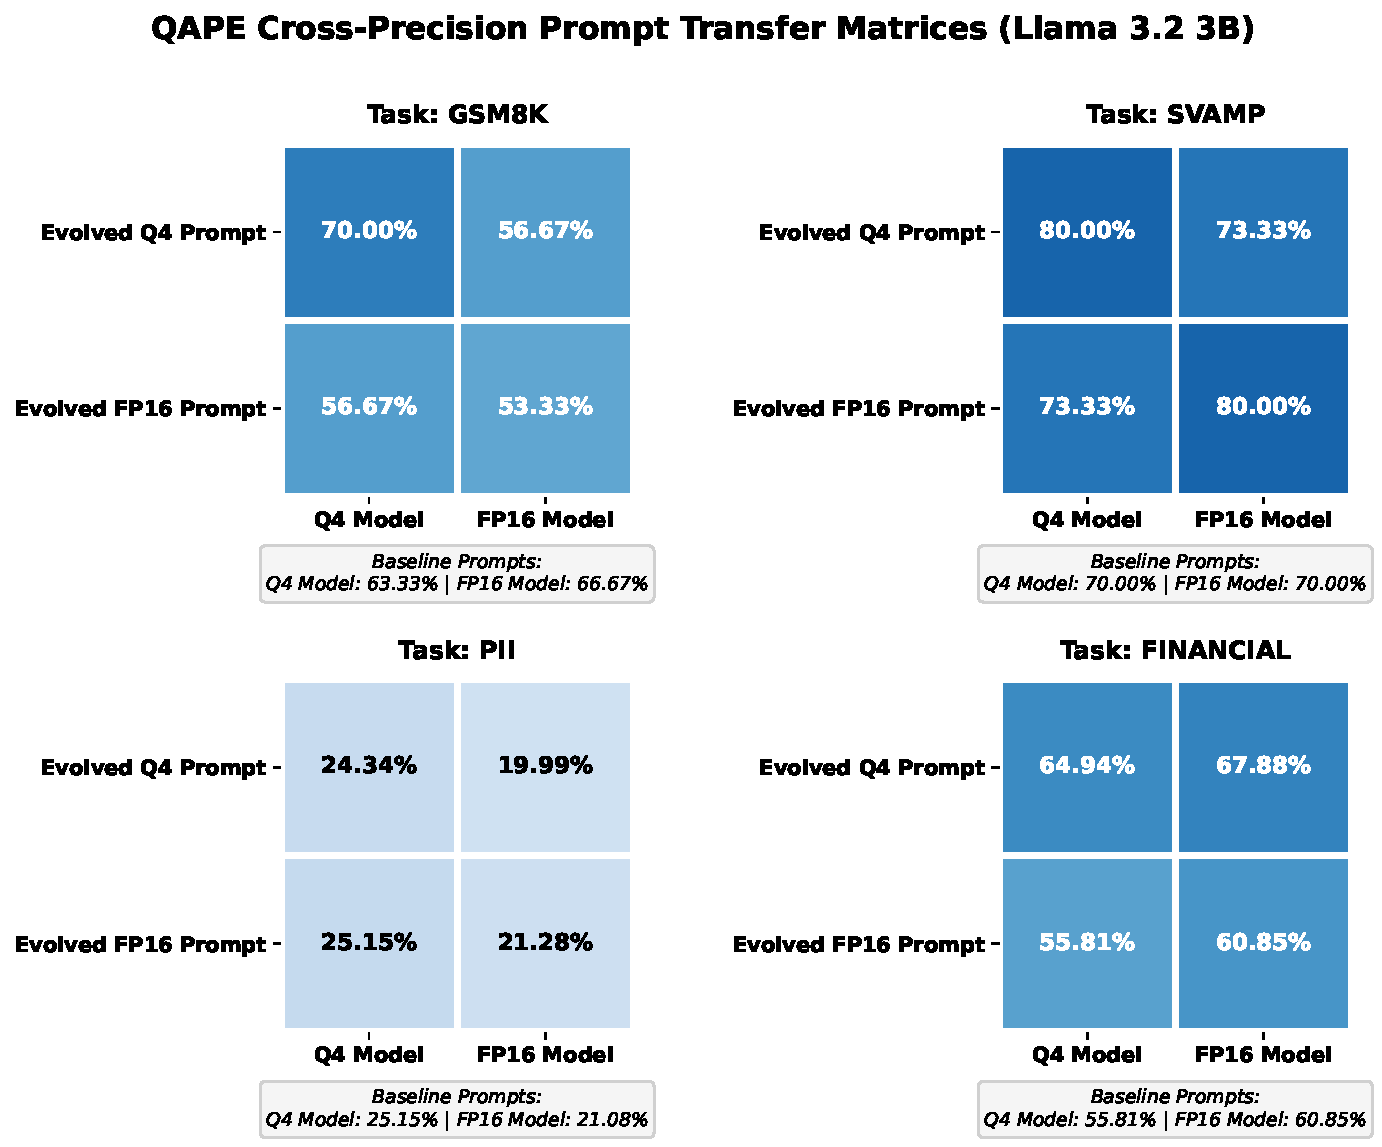
\includegraphics[width=\columnwidth]{prompt_transfer_matrix.pdf}
\caption{QAPE cross-precision prompt transfer matrices across the four benchmarks on Llama-3.2-3B. The diagonal cells represent direct optimization, while off-diagonals represent transfer across precision boundaries.}
\label{fig:transfer-matrix}
\end{figure}

\begin{table*}[t]
\centering
\small
\begin{tabular}{llccc}
\toprule
\textbf{Task} & \textbf{Target Model (Precision)} & \textbf{Baseline Prompt} & \textbf{Evolved Q4 Prompt} & \textbf{Evolved FP16 Prompt} \\
\midrule
\textbf{GSM8K} & \texttt{llama3.2} (Q4) & 63.33\% & \textbf{70.00\%} & 56.67\% \\
               & \texttt{llama3.2} (FP16) & \textbf{66.67\%} & 56.67\% & 53.33\% \\
\midrule
\textbf{SVAMP} & \texttt{llama3.2} (Q4) & 70.00\% & \textbf{80.00\%} & 73.33\% \\
               & \texttt{llama3.2} (FP16) & 70.00\% & 73.33\% & \textbf{80.00\%} \\
\midrule
\textbf{PII}   & \texttt{llama3.2} (Q4) & \textbf{25.15\%} & 24.34\% & \textbf{25.15\%} \\
               & \texttt{llama3.2} (FP16) & 21.08\% & 19.99\% & \textbf{21.28\%} \\
\midrule
\textbf{Financial} & \texttt{llama3.2} (Q4) & 55.81\% & \textbf{64.94\%} & 55.81\% \\
                   & \texttt{llama3.2} (FP16) & 60.85\% & \textbf{67.88\%} & 60.85\% \\
\bottomrule
\end{tabular}
\caption{Cross-precision transfer matrix evaluating prompts evolved on Q4 vs. FP16 targets on Llama-3.2-3B.}
\label{tab:transfer-matrix}
\end{table*}

\subsection{Key Observations on Transferability}
\begin{enumerate}
    \item \textbf{Precision Specialization:} On reasoning tasks (GSM8K and SVAMP), prompts exhibit strong numerical precision specialization. A prompt optimized on Q4 achieves peak performance on Q4 (80.00\%) on SVAMP, but transferring it to FP16 drops accuracy to 73.33\%. Conversely, the FP16 evolved prompt achieves 80.00\% on FP16, but drops to 73.33\% when run on Q4.
    \item \textbf{Structured Extraction Transferability:} For the structured extraction task (Financial NER), prompt transfer is highly asymmetrical and beneficial. The prompt evolved on Q4 transfers exceptionally well to FP16, achieving \textbf{67.88\%} (beating the FP16 baseline of 60.85\%). This suggests that prompts optimized to force strict formatting constraints in highly quantized models also stabilize entity parsing in full-precision models.
\end{enumerate}

\section{Discussion}
Our cross-precision transfer results reveal two prominent architectural insights:

\paragraph{Mechanisms of Precision Specialization}
The drop in accuracy observed when transferring evolved prompts across precision boundaries (e.g., Q4 prompts on FP16 weights, and vice-versa) points to \textit{precision-dependent prompt specialization}. When optimizing on quantized models, the genetic mutation loop selects for prompts that bypass the numerical noise introduced by quantization grids. These evolved prompts often utilize specific vocabulary distributions and syntactic patterns that stabilize internal attention weights. When executed on full-precision weights (FP16), these specialized formatting and lexical constraints are no longer required and end up over-constraining the model's natural reasoning paths, leading to a performance degradation compared to directly optimized prompts.

\paragraph{Asymmetric Formatting Resilience in Structured Extraction}
Unlike mathematical reasoning tasks, structured information extraction tasks (such as Financial NER) demonstrate high resilience to cross-precision prompt transfer, showing an asymmetric benefit. Prompts evolved on the Q4 model transfer exceptionally well to FP16 targets (outperforming baseline scores by 7.03\%). In low-parameter quantized SLMs, maintaining formatting constraints (e.g., producing valid JSON arrays) is a primary bottleneck. Consequently, the Q4 evolutionary loop acts as a strict structural filter, selecting prompts with concrete JSON schemas and output syntax rules. Because formatting stability is a shared requirement across all precision levels, these highly constrained templates serve as robust anchors for the full-precision weights, yielding high transfer performance.

\section{Conclusion}
We presented QAPE, demonstrating that prompt optimization is a viable, compute-efficient method to reclaim reasoning and extraction capabilities in quantized SLMs. Our cross-precision transfer evaluations reveal that prompts specialize to the quantization-induced noise of their target precision. In future work, we plan to construct joint multi-precision objective functions to evolve prompts that are robust across both quantized and full-precision weights.

\section*{Limitations}
Although QAPE successfully recovers quantization-induced performance drops, this study has several limitations:
\begin{enumerate}
    \item \textbf{Evaluation Scale:} Due to local CPU and memory constraints on edge devices, final evaluations were conducted on a subset of 30 test samples per task. While these show clean statistical gains, larger validation sets would provide tighter confidence bounds.
    \item \textbf{Hardware Scope:} Experiments were conducted exclusively on Apple Silicon (M3) unified memory architectures. While this represents a standard edge deployment target, the performance and latency characteristics of quantized SLMs under local execution are known to vary across other CPU and mobile hardware families.
    \item \textbf{Model Families:} We evaluated sub-3B parameter instruction-tuned models. The prompt specialization behaviors observed here may differ in larger scale models (e.g., 8B or 70B), where representation capacity is higher and quantization-induced drift is less severe.
\end{enumerate}

\section*{Ethics Statement}
This research respects privacy and user data protections. All datasets used (GSM8K, SVAMP, Cleanlab PII, and Financial NER) are publicly available academic datasets. For PII anonymization tasks, the synthetic evaluation splits contain mock data rather than real personal information, presenting zero risk of disclosure. The computational footprints of our prompt evolution experiments are small (sub-3B models run locally on a single consumer device), aligning with green AI goals by avoiding energy-intensive GPU cluster training.

\bibliography{custom}
\bibliographystyle{acl_natbib}

\end{document}
